%%%%%%%%%%%%%%%%%%%%%%%%%%%%%%%%%%%%%%%%%%%%%%%%%%%%%%%%%%%%%%%%%%%%%%
%%%%%%%%%%%%%% Pacotes básicos obrigatório        %%%%%%%%%%%%%%%%%%%%
%%%%%%%%%%%%%%%%%%%%%%%%%%%%%%%%%%%%%%%%%%%%%%%%%%%%%%%%%%%%%%%%%%%%%%

\documentclass[12pt]{article} 
\usepackage[utf8x]{inputenc}
\usepackage[brazilian]{babel}
\usepackage{fontenc}
\usepackage{graphicx} 
\usepackage{xcolor}


%%%%%%%%%%%%%%%%%%%%%%%%%%%%%%%%%%%%%%%%%%%%%%%%%%%%%%%%%%%%%%%%%%%%%%
%%%%%%%%%%%%%% Alguns Pacotes que podemos utilizar%%%%%%%%%%%%%%%%%%%%
%%%%%%%%%%%%%%%%%%%%%%%%%%%%%%%%%%%%%%%%%%%%%%%%%%%%%%%%%%%%%%%%%%%%%%

\usepackage{indentfirst} %identa o primeiro paragrafo da seção
%\usepackage{pdflscape} % se quiser colocar uma figura na pagina deitada

%se quiser alterar as bordas da página
% \usepackage[bottom=3cm,top=3cm,left=3cm,right=3cm]{geometry} 
\usepackage[pdftex]{hyperref} %permitir \url clicável nos links
% \usepackage{subfig}

%%%%%%% Para colocar a logo da ufc na primeira página %%%%%%%%%%%%%%%%
\usepackage{wallpaper} 
\usepackage[absolute]{textpos}

%%%%%%%%%%%%%%%%%%%%%%%%%%%%%%%%%%%%%%%%%%%%%%%%%%%%%%%%%%%%%%%%%%%%%%
%%%%%%%%%%%%%% Configurando pacote para bordas  %%%%%%%%%%%%%%%%%%%%%%
%%%%%%%%%%%%%%%%%%%%%%%%%%%%%%%%%%%%%%%%%%%%%%%%%%%%%%%%%%%%%%%%%%%%%%
\usepackage[framemethod=TikZ]{mdframed} % para os frames
\mdfsetup{%
	%middlelinecolor=red,
	middlelinewidth=2pt,
	%backgroundcolor=red!20,
	%roundcorner=10pt
}

%%%%%%%%%%%%%%%%%%%%%%%%%%%%%%%%%%%%%%%%%%%%%%%%%%%%%%%%%%%%%%%%%%%%%%
%%%%%%%%%%%%%% Configurando pacote para cabeçalho %%%%%%%%%%%%%%%%%%%%
%%%%%%%%%%%%%%%%%%%%%%%%%%%%%%%%%%%%%%%%%%%%%%%%%%%%%%%%%%%%%%%%%%%%%%
\usepackage{fancyhdr}
\pagestyle{fancy}
\fancyhf{}
\lhead{Fundamentos de Programação}
\rhead{UFC - Quixadá}
\fancyfoot[R]{\thepage}
\rfoot{Page \thepage}


%%%%%%%%%%%%%%%%%%%%%%%%%%%%%%%%%%%%%%%%%%%%%%%%%%%%%%%%%%%%%%%%%%%%%%
%%%%%%%%%%%%%% Configurando pacote para códigos   %%%%%%%%%%%%%%%%%%%%
%%%%%%%%%%%%%%%%%%%%%%%%%%%%%%%%%%%%%%%%%%%%%%%%%%%%%%%%%%%%%%%%%%%%%%
\usepackage{listings}
\lstset{
	%language=java,
	language=c++,
	keywordstyle=\bfseries\ttfamily\color[rgb]{0,0,1},
	identifierstyle=\ttfamily,
	commentstyle=\color[rgb]{0.133,0.545,0.133},
	stringstyle=\ttfamily\color[rgb]{0.627,0.126,0.941},
	showstringspaces=false,
	basicstyle=\small,
	tabsize=2,
	breaklines=true,
	frame=single
}


%%%%%%%%%%%%%%%%%%%%%%%%%%%%%%%%%%%%%%%%%%%%%%%%%%%%%%%%%%%%%%%%%%%%%%
%%%%%%%%%%%%%% Definindo Atalhos %%%%%%%%%%%%%%%%%%%%%%%%%%%%%%%%%%%%%
%%%%%%%%%%%%%%%%%%%%%%%%%%%%%%%%%%%%%%%%%%%%%%%%%%%%%%%%%%%%%%%%%%%%%%


\newcommand{\code}[1]{\lstinline|#1|} %% para codigos inline
\newcommand{\ita}[1]{\textit{#1}}  %% para italico
\newcommand{\bold}[1]{\textbf{#1}} %% para negrito
\newcommand{\note}[1]{\footnote{#1}} %% para anotações laterais
\newcommand{\caps}[1]{\textbf{#1}} %% para CAPS

%%%%%%%%%%%%%%%%%%%%%%%%%%%%%%%%%%%%%%%%%%%%%%%%%%%%%%%%%%%%%%%%%%%%%%
%%%%%%%%%%% Escolha da fonte     %%%%%%%%%%%%%%%%%%%%%%%%%%%%%%%%%%%%%
%%%%%%%%%%%%%%%%%%%%%%%%%%%%%%%%%%%%%%%%%%%%%%%%%%%%%%%%%%%%%%%%%%%%%%
% Deixe as duas comentadas para usar o default Helvetica e Palatino
%\usepackage{lmodern}
%\usepackage{txfonts}



\begin{document}

\ThisULCornerWallPaper{1}{./imagens/header}
\begin{textblock}{15}(0.4, 0.4)
	\noindent
	\begin{center}
		\LARGE{\bf{QXCode - Quixadá Coding Team}}\\
		\large{\bf{Fundamentos de Programação}} \\
		\large{\bf{\today}}
	\end{center}
\end{textblock}

\title{\bf{Blackjack \\ Laboratório Prático}}

\author{
	David Sena Oliveira\thanks{sena.ufc@gmail.com}
}

\date{}

\maketitle
\thispagestyle{empty}

%#################################################################
%#################################################################
%#################################################################
%#################################################################
\section{Introdução}

Nessa prática nós vamos trabalhar apenas com:
\begin{itemize}
	\item Estruturas de seleção,
	\item Vetores
	\item Laço,
	\item Funções.
\end{itemize}

Vamos trabalhar com C++ nesse laboratório.

\section{Primeiras definições}

A primeira decisão é como vamos definir uma carta. Podemos utilizar:

\begin{itemize}
	\item Uma variável \bold{int} de 1 a 13 representando as cartas.
	\item Uma variável \bold{char} com A1234567890JQK sendo nossas cartas.
\end{itemize}

Basicamente precisamos ser capazes de sortear, imprimir e manipular nossas
cartas.  As duas primeiras opções são boas. Vamos escolher definir a carta como
um inteiro.  \footnote{Sugiro que você tente fazer com \bold{char} por diversão
depois.}

\subsection{Sorteando a carta}

Nosso primeiro objetivo é fazer uma função que gere aleatóriamente uma carta
válida.  Por enquanto, não vamos montar o baralho todo. Vamos apenas gerar um
valor válido aleatório entre 1 e 13.

Em C e C++ você pode usar a função \code{rand()} para gerar um número aleatório.

\begin{mdframed}[nobreak=true]
	\centering{rand() em C++}
	\begin{lstlisting}
	#include <iostream>
	#include <cstdlib> //para usar rand() e srand()
	#include <ctime> //para utilizar time()

	int main(){
		srand(time(NULL)); //inicia a aleatoriedade
	int num = rand() % 5; // 0, 1, 2, 3 ou 4
	std::cout << num << std::endl;
	return 0;
}
	\end{lstlisting}
\end{mdframed}

\begin{figure}[h]
	\centering
	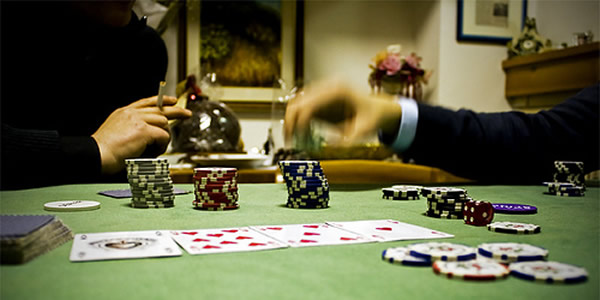
\includegraphics{imagens/mesa}
\end{figure}

Você só precisa chamar a função \code{srand(time(NULL))} uma única vez no seu
código. Normalmente, durante a inicialização das variáveis. Faça uma função
\code{int sortear_carta();}que gera um número entre 1 e 13 usando \code{rand}.
Teste pra ver se ela funciona mesmo e se a cada vez que seu código é executado,
ela gera um valor diferente.

\section{Mostrando a carta}

Precisamos ser capazes de mostrar o número como uma carta. Se nossa carta é um
$12$, queremos imprimir $Q$ e não o 12. Podemos fazer isso de duas formas.
A primeira é criar uma função que recebe o número inteiro e retorna uma
\code{string}. A segunda é colocando todas as cartas em um vetor de strings e
utilizar o índice para pegar as cartas.


\begin{mdframed}[nobreak=true]
	\centering{Mostrando as cartas}
	\begin{lstlisting}
	#include <iostream>
	#include <vector>

	//Primeira forma
	string pegar_nome(int carta){
		if(carta == 1)
			return "A";
		if(carta > 1 && carta < 11)
			return std::to_string(carta);
		//...
	}

	//Segunda forma:  
	vector<string> nomes{"", "A", "2", ..., "Q", "K"};
	string pegar_nome(int carta){
		return nomes[carta];
	}
	\end{lstlisting}
\end{mdframed}

O método \code{string to_string(value)} to C++ recebe um int, char, float,
double e retorna uma string. 

\subsection{Calculando mão de cartas}

Vai ser útil se você tiver uma função que recebe a carta e retorna o valor.

%\begin{mdframed}[nobreak=true]
	\begin{lstlisting}
	int pegar_valor(int carta){
		if(carta == 1)
			return 11;
		else if( //termine o codigo ok...
	}
	\end{lstlisting}
%\end{mdframed}

Para nós, o A vale 11, a não ser que isso estoure a mão do jogador. Mas por favor,
não faça um \code{if} para cada carta, ok? Observe a lógica e veja que 10, J, Q
e K, possuem o mesmo valor, portanto podem ficar no mesmo \code{if}. Os números
de 2 a 9 também podem ficar no mesmo \code{if}.

\subsection{Calculando a mão}

Agora o caldo engrossa! Aqui temos provavelmente a parte mais interessante do
código. Nosso objetivo é assumir que o A vale 11 e calcular o valor da mão. Ao
mesmo tempo contamos quantos As tem na nossa mão. Após termos o total, se ele
passar de 21, vamos descontando nossas cartas As, para fazer o valor baixar.

\begin{mdframed}[nobreak=true]
	\centering{Pseudocódigo para calcular o valor de uma mao}
	\begin{lstlisting}
	int valor_mao(vector<int> mao){
		total = 0
		n_as = 0
		Para cada carta na mao:
			incremente total do valor da carta
			Se a carta for um A:
				n_as aumenta de 1
		Enquanto o total > 21 e n_as > 0:
			decrementa total de 10
			decremente n_as de 1
		retorne total
	}
	\end{lstlisting}
\end{mdframed}

Perceba que fazer o A voltar de 11 para 1 significa retirar 10 pontos do valor
da mão. Você pode fazer isso, quantas vezes você precisar(enquanto tiver
estourado) e ainda tiver A pra trocar.

\subsection{Vamos JOGAAAAAAAAARRRRRR!!!}

O dealer\note{O funcionário que coordena a mesa} pede uma carta
para mesa e duas para o jogador deixando todas viradas para cima. O jogador vai
pedindo cartas à mesa. Seu objetivo é chegar o mais perto que puder de ter uma
mão com valor 21. Se ele passar de 21 ele automaticamente perde. Se ele fizer
exatos 21 pontos ele ganha. 

Após o jogador parar sua jogada, supondo que ele não estourou o limite, a
mesa(máquina) vai puxar as cartas para tentar vencer o jogador. A mesa tem a
vantagem do empate. Se ela fizer a mesma pontuação do jogador ela ganha. Se ela
estourar, ela perde. \note{No nosso modelo, a mesa ou ganha ou estoura, porque
ela não vai se contentar em perder.}

Vou lhe ajudar com a lógica ok?

\begin{mdframed}[nobreak=true]
	\centering{Pseudocódigo para lógica do jogo}
	\begin{lstlisting}
		mao_mesa comeca vazia
		mao_jogador comeca vazia
		puxa uma carta para mao_mesa
		puxa duas cartas para mao_jogador
		PARAR = false
		Enquanto jogador nao PARAR ou nao estourar:
			mostrar maos
			pergunta opcao ao jogador
			se opcao for pedir
				puxa carta para mao_jogador
			senao se opcao for parar
				PARAR = true
		Enquanto mesa nao ganhar ou estourar
			puxar carta para mesa
			mostrar maos

	\end{lstlisting}
\end{mdframed}

Sugiro que crie uma função que mostre a mão de um jogador. Algo como \code{string mostrar_mao(vector<int> mao)}.
A saída pode ser parecida \code{Total 17 [2 A 4 K]}. A seguir, um exemplo de possível aparência do jogo.

\begin{mdframed}[nobreak=true]
	\centering{Exemplo: Jogador perdendo.}

	\begin{verbatim}
	Iniciando Rodada:
	# Mesa recebe  7 - Total  7 [ 7 ]
	# Voce recebe  A - Total 11 [ A ]
	# Voce recebe  2 - Total 13 [ A 2 ]
	Pedir = 1, Parar = 2 
	>> 1

	# Voce recebe  3 - Total 16 [ A 2 3 ]
	Pedir = 1, Parar = 2 
	>> 2

	# Mesa recebe  2 - Total  9 [ 7 2 ]
	# Mesa recebe  7 - Total 16 [ 7 2 7 ]
	# Mesa (16), Voce (16)
	Voce perdeu!
	\end{verbatim}
\end{mdframed}

\section{Melhorias}

Deixo aqui algumas sugestões pra sua diversão.
\begin{enumerate}
	\item Implementar um laço no qual o jogador continua jogando até que decida parar.
	\item Implementar um esquema de apostas no qual o jogador decide quanto quer apostar antes da rodada. O jogador pode começar com uma quantia fixa de dinheiro. Se ele ganhar a rodada, o dinheiro é adicionado na conta dele. Se ele perde, então, a, um, então ele perde.
	\item Montar um ou dois baralhos com as cartas e embaralhar. Retirar então as cartas, e após a rodada, elas vão para o montante até que o baralho termine. 
	\item Implementar o jogo com mais de um jogador. Nele, a mesa vai precisar de regras um pouco diferentes. Consulte a wiki sobre Blackjack para entender mais.
\end{enumerate}

\end{document}
